\documentclass[12pt,a4paper]{report}

\usepackage[italian]{babel}
\usepackage{newlfont}
\usepackage{graphicx,  caption}
\usepackage{version}
\usepackage{chngcntr}
%\usepackage{float}
\usepackage{listings}

\usepackage{floatrow}
\usepackage{float}

\usepackage{booktabs,dcolumn}

\textwidth=450pt\oddsidemargin=0pt

\begin{document}

\begin{titlepage}
\begin{center}
{{\Large{\textsc{Alma Mater Studiorum $\cdot$ Universit\`a di
Bologna}}}} \rule[0.1cm]{15.8cm}{0.1mm}
\rule[0.5cm]{15.8cm}{0.6mm}
{\small{\bf DIPARTIMENTO DI INFORMATICA – SCIENZA E INGEGNERIA\\
Corso di Laurea in Ingegneria e Scienze Informatiche }}
\end{center}
\vspace{15mm}
\begin{center}
{\LARGE{\bf PARALLELIZZAZIONE SU GPU}}\\
\vspace{3mm}
{\LARGE{\bf ALGORITMO MARCHING SQUARES}}\\
\vspace{3mm}
{\LARGE{\bf PER APPLICAZIONE INDUSTRIALE}}\\
\vspace{25mm}

Elaborato in:\\
High Performance Computing\\
\end{center}
\vspace{25mm}
\par
\noindent
\begin{minipage}[t]{0.47\textwidth}
{\large{\bf Relatore:\\
Chiar.mo Prof.\\
Moreno Marzolla\\}}
{\large{\bf \\Correlatore:\\
Dott.\\
Matteo Roffilli}}
\end{minipage}
\hfill
\begin{minipage}[t]{0.47\textwidth}\raggedleft
{\large{\bf Presentata da:\\
Alessandro Sciarrillo}}
\end{minipage}
\vspace{30mm}
\begin{center}
{\large{\bf 
%Sessione\\%inserire il numero della sessione in cui ci si laurea
Anno Accademico 2022/2023}}%inserire l'anno accademico a cui si Ë iscritti
\end{center}
\end{titlepage}

\tableofcontents

\chapter{Abstract}
% una vista rapida della tesi 1/2 facciate, cosa si andrà a fare, quale è il problema, cosa si fa per risolverlo e quali risultati si otterranno. 
% keyword: cosa siANDRà a fare, OTTERREMO
Marching Squares(MS) é un algoritmo per la generazione di contorni in un campo scalare bidimensionale che viene ampiamente utilizzato nel Machine Vision in ambito industriale. Nella applicazione pratica in questione viene utilizzato su fotografie scattate da macchine per la selezione automatica della frutta per trovare i contorni di aree dell'immagine dove vengono riconosciuti dei difetti nel frutto. L'algoritmo viene applicato all'output di una CNN (Convolutional Neural Network) che é composto da una mappatura dei pixel dell'immagine in input nella rispettiva probabilità di appartenere ad una certa classe di difetto, vengono costruiti i contorni delle aree che hanno una probabilità maggiore di una certa soglia di contenere una certa classe. Le classi di difetto sono ad esempio: marcio, ruggine, danno da grandine fresca, danno da grandine cicatrizzato, danno da raccolta, danno da trasporto ecc.. \newline
Per ogni frutto che deve essere smistato correttamente dalle macchine in base alle sue condizioni vengono scattate più foto mentre viene trasportato su dei rulli che lo fanno roteare e permettono quindi alle fotocamere di raccogliere un insieme di scatti in cui il frutto é stato catturato in tutte le sue facce. Per ognuna delle foto scattate al frutto vengono generate delle matrici di probabilità per ogni classe di difetto, il risultato del processo di selezione é quindi l'insieme delle immagini dei vari lati di quel preciso frutto con i vari difetti racchiusi da un contorno che li identifica. \newline 
La costruzione di questo contorno viene attualmente effettuato da Python tramite il metodo \verb|findContours| della libreria skimage che utilizza un'implementazione seriale dell'algoritmo Marching Squares, lo scopo di questa ricerca é di implementare una versione parallela su GPU dell'algoritmo in modo da ridurre i tempi di esecuzione che risultano un fattore di importanza fondamentale.  Infatti ogni frazione di secondo risparmiata può essere utilizzata per aumentare il numero di frutti classificati in un'unità di tempo o per dedicare quel tempo ad altre elaborazioni utili a migliorare il risultato. 
Il metodo \verb|findContours| di skimage é scritto in Python ma la parte principale in cui utilizza MS é stata scritta in Cython (codice Python-like che viene compilato in codice C) per migliorare i tempi di esecuzione, può essere quindi considerata come una versione seriale già particolarmente ottimizzata. \newline L'obbiettivo è di parallelizzare proprio la stessa parte dell'algoritmo che skimage mantiene in Cython che è anche l'unica porzione di codice parallelizzabile dell'algoritmo MS. \newline
Le principali strategie che verranno esplorate sono:
\begin{itemize}
\item utilizzo dell'ultima versione di nvc++ per la parallelizzazione in fase di compilazione del codice Cython
% \item utilizzo delle direttive OpenMP per la parallelizzazione del codice C derivato dal codice Cython
\item utilizzo delle API Cuda-Python per il lancio di kernel Cuda (scritti manualmente) da Python 
\end{itemize}
Il metodo migliore che verrà poi utilizzato per la soluzione finale sarà quello che sfrutta le API Cuda-Python e i kernel Cuda scritti manualmente, riuscirà infatti ad ottenere uno Speedup di circa x5**[NOTA: sulla mia macchina,  attendo test su server azienda per aggiornare valore e inserire specifiche macchina] %TODO scrivere specifiche macchina
 rispetto al corrispondente codice seriale della libreria skimage. Verrà anche analizzato l'overhead nel lancio dei kernel Cuda introdotto da Python rispetto a una versione scritta in C. \newline
Nella soluzione finale viene inoltre implementata una elaborata versione parallela di exlusive scan composta da più kernel che risulta di particolare interesse nell'ambito dell'High Performance Computing.

\chapter{Introduzione alla programmazione Parallela}
% guardare altre tesi per vedere in che ordine metterlo
% valutare se tenerlo o meno

% introdurre almeno il signifficato di Device Host e blocco thread Cuda core

\chapter{Introduzione e Analisi del Problema}
\section{Introduzione}
% spiegare il problema e la sua utilità, obbiettivo
\subsection{Marching Squares (MS)} %valutare di farlo diventare capitolo
L'algoritmo Marching Squares genera contorni per un campo scalare a due dimensioni, data una matrice di valori e una soglia é in grado di trovare un insieme di segmenti che delimitano le aree della matrice in cui il valore contenuto dalle singole celle é maggiore della soglia data. \newline
Una delle elaborazioni più utilizzate viene effettuata considerando separatamente ogni gruppo di quattro elementi della matrice disposti a forma di quadrato, ognuno di questi quadrati può ricadere in uno di sedici diversi casi possibili ben definiti. Per definire a quale tipo appartiene un certo quadrato bisogna prima binarizzare i valori dei quattro spigoli in base alla soglia data, la posizione dei valori negli spigoli é importante poiché i sedici casi sono definiti con un'orientazione ben precisa. Nella figura 3.1 é possibile vedere una generica rappresentazione dei sedici casi possibili nella versione più comune di Marching Squares.
In questa versione vengono considerate delle Isolinee ma esiste anche una variante in cui vengono considerate delle Isobande che sono costruite con l'aggiunta alle barre di contorno di upper e lower thresholds come rappresentato nell'immagine 3.2. \newline Esistono anche versioni che invece dei quadrati utilizzano triangoli e vengono applicate per l'individuazione di meshes triangolari.
\begin{figure}[H]
    \centering
    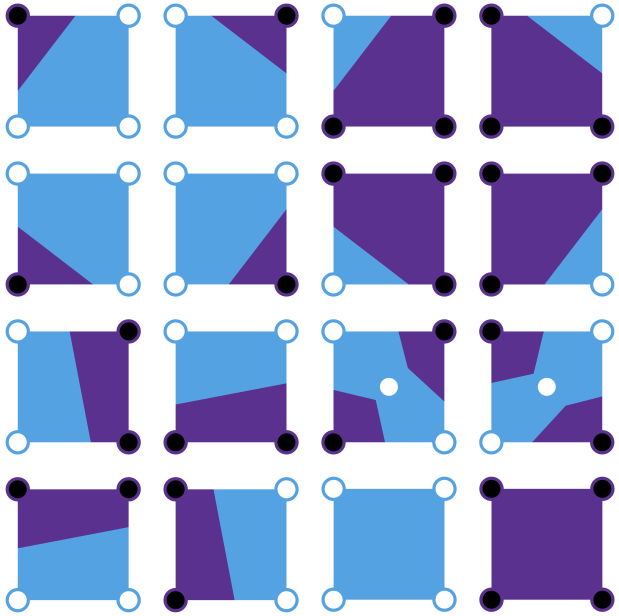
\includegraphics[scale=0.32]{img/Marching_squares_isolines.svg.png}
    \caption{Sedici casi possibili in cui possono ricadere i quadrati composti dai quattro valori.}
\end{figure}
\begin{figure}[H]
    \centering
    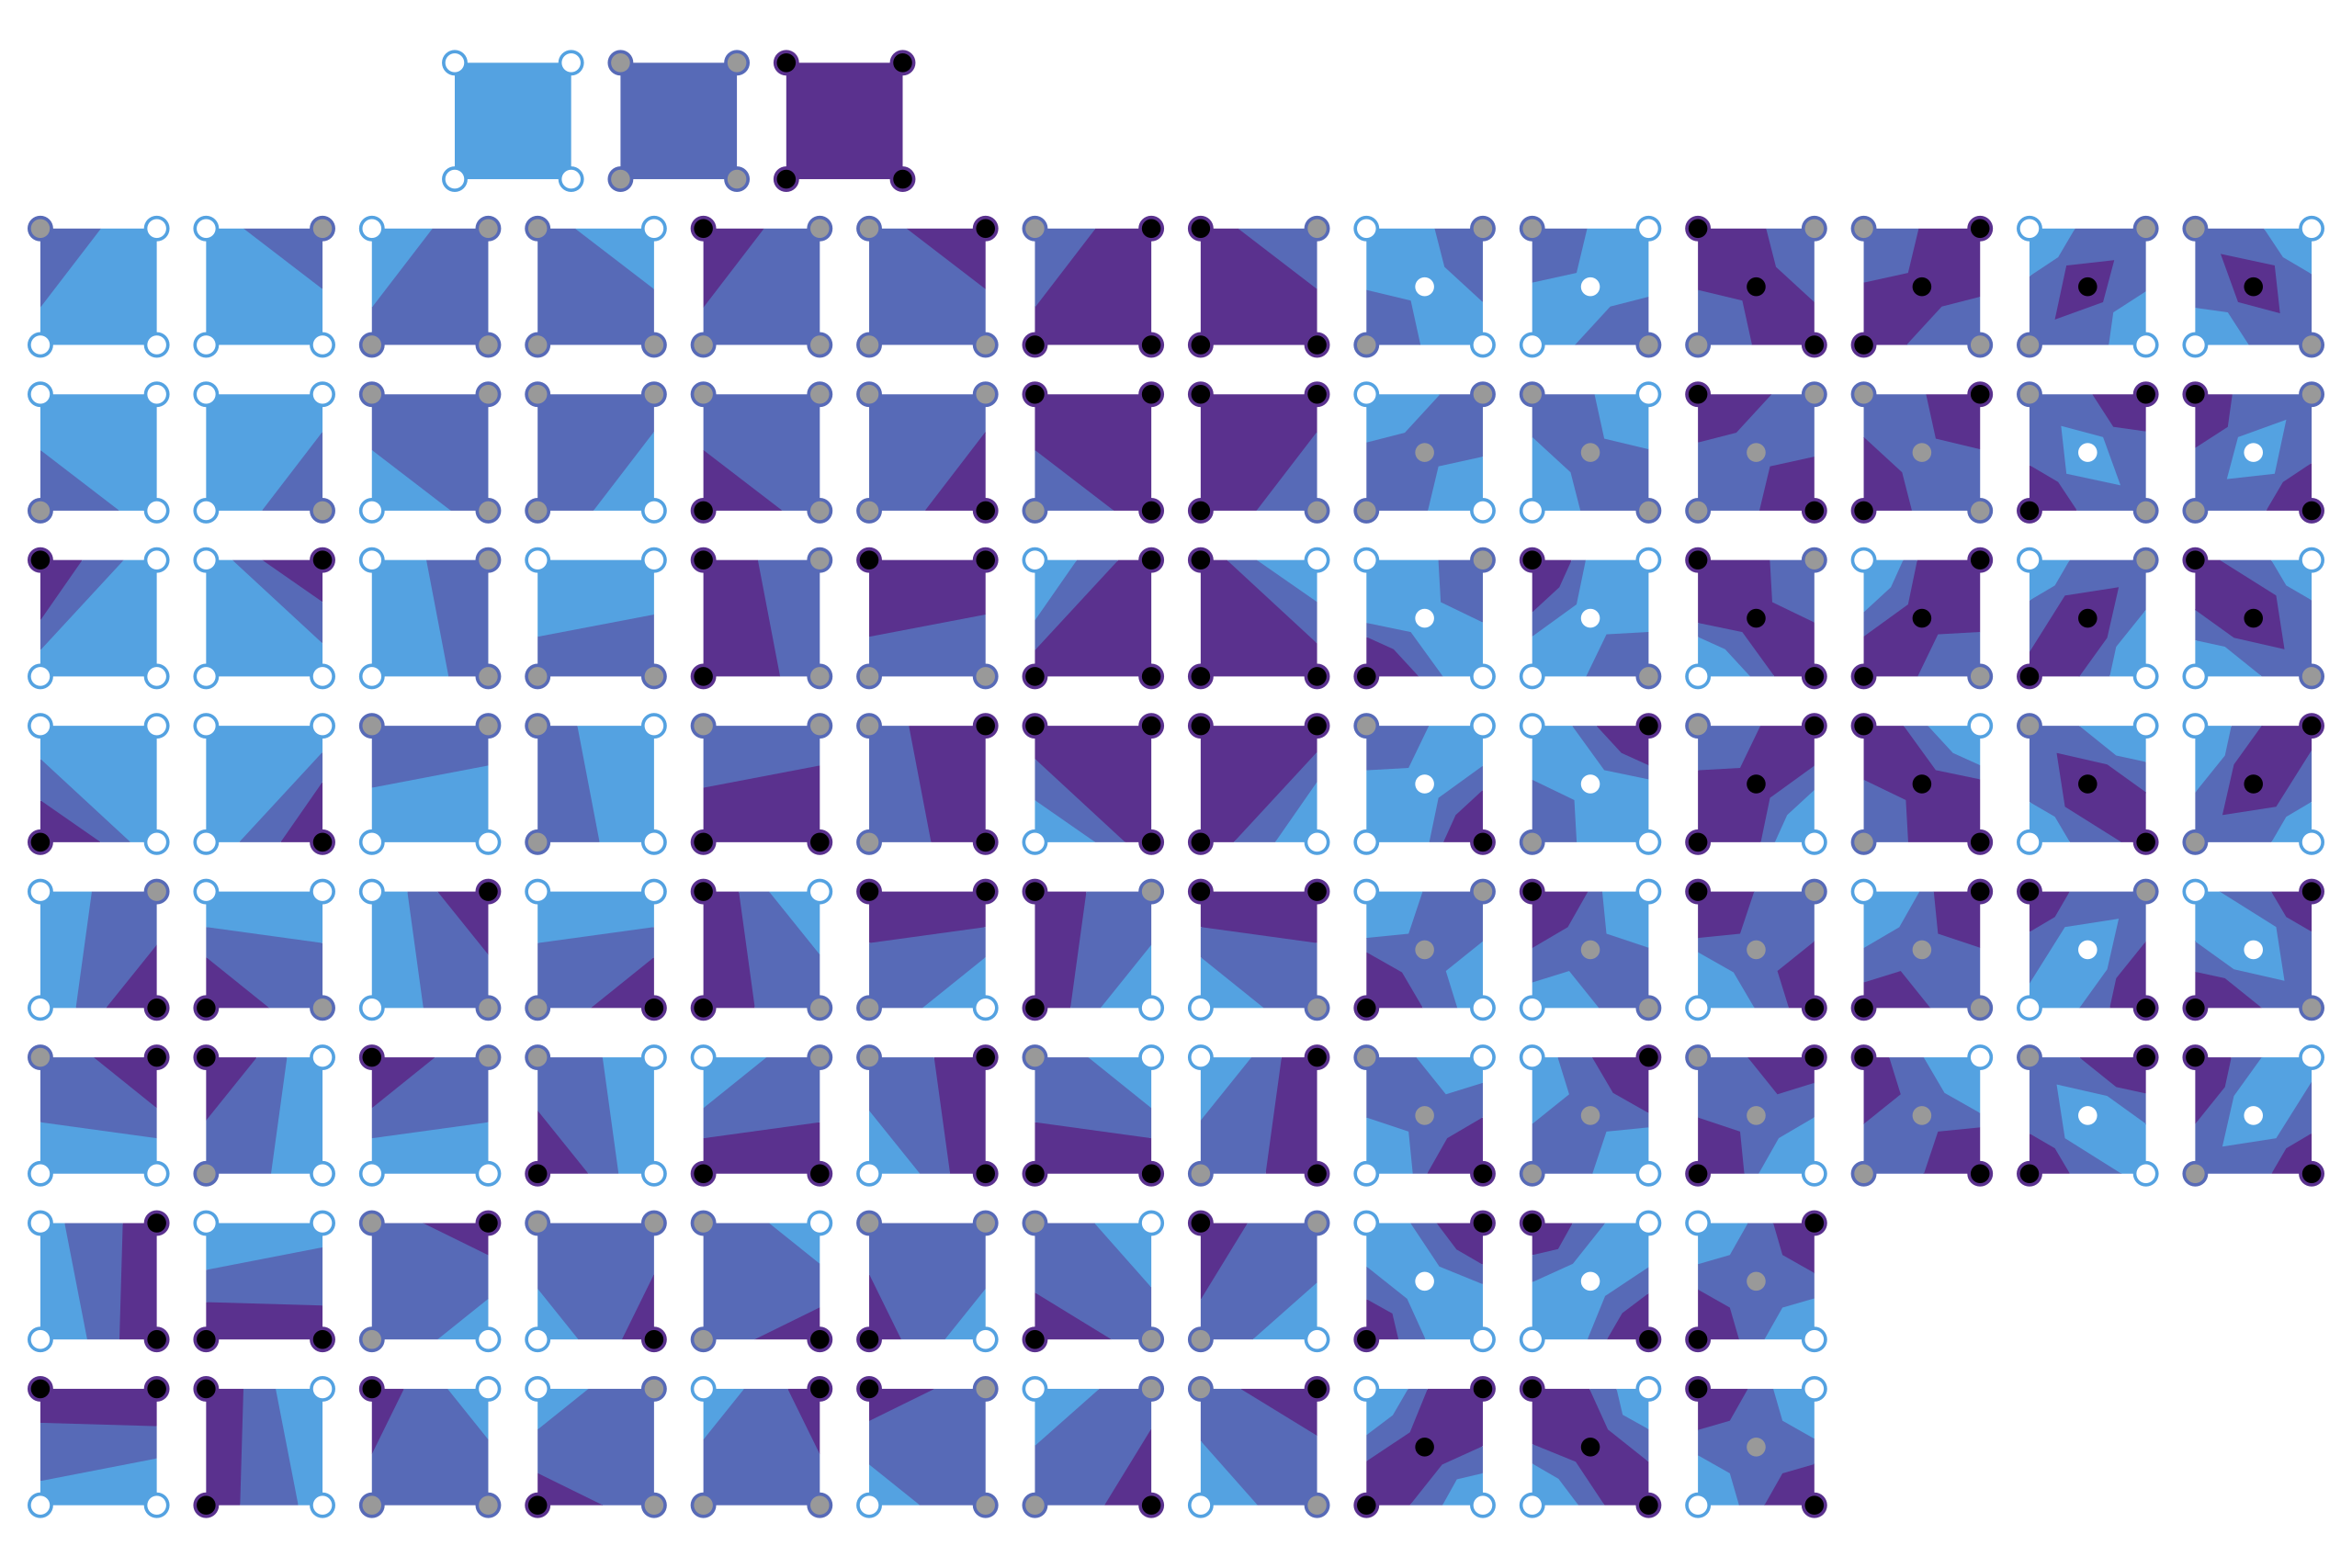
\includegraphics[scale=0.17]{img/Marching_squares_isobands.svg.png}
    \caption{Casi possibili nella versione con isobande in cui possono ricadere i quadrati composti dai quattro valori.}
\end{figure}

%embarrassingly parallel
% problema di classificazione tipo in modo indipendente ma ricostruzione contorno unito in modo seriale/congiunto
L'algoritmo é embarrassingly parallel per quanto riguarda la classificazione per tipo di ogni cella (quadrato con valori negli spigoli) poiché puó essere svolta in modo indipendente tra le celle. \newline
La fase di ricostruzione dei contorni invece può essere svolta sia in parallelo che in seriale utilizzando tecniche e modalità differenti che dipendono dall'utilizzo finale a cui il codice é destinato. \newline
%utilizzi reali, utilitá
MS è utilizzato per molte applicazioni pratiche in settori di particolare interesse come ad esempio:
\begin{itemize}
\item Computer Graphics per generare immagini 3D da dati 2D.
\item Rilevamento remoto in immagini satellitari o radar.
\item Medicina per analizzare scansioni CT o immagini MRI dove possono essere identificare anomalie come tumori.
\item Scienze naturali per l'analisi di dati meteorologici e oceanici nell'identificazione di aree di pioggia o di correnti forti.
\item Cartografia per la generazione di mappe relative a paesi o città da dati 2D.
\end{itemize}

\subsection{Problema Reale}
Bioretics è l'azienda con cui è stara svolta la ricerca, uno dei settori in cui opera è quello della selezione automatica della frutta. La selezione della frutta è un processo svolto in questo caso da macchine dotate di rulli e fotocamere, i frutti entrano nella macchina all'interno di tazze e vengono fatti roteare da dei rulli in modo da poter acquisire con delle camere fissate all'interno della macchina delle immagini di tutta la superficie dei frutti. Le immagini scattate per ogni frutto vengono processate e passate ad una CNN che restituisce delle matrici della stessa dimensioni delle immagini scattate, una per ogni classe di difetto che si vuole valutare, che hanno come valore la probabilità che il rispettivo pixel appartenga a quella classe. \newline

L'azienda offre in sostanza un prodotto software che viene eseguito da macchine per la selezione della frutta e include l’utilizzo dell'algoritmo Marching Squares (MS). La sfida proposta dall'azienda è quella di ridurre i tempi di esecuzione di MS che è utilizzato nella fase di segmentazione dei difetti.
Le macchine per la selezione gestiscono un flusso di circa 10 frutti al secondo, ne consegue che ci sia approssimativamente 0.1s a disposizione per ogni frutto. Quindi un’implementazione parallela dell’algoritmo MS, che riesca a ottenere uno speedup anche solo di 1.1 sarebbe considerato un risultato positivo per l’azienda.
Scendendo più nel merito degli aspetti tecnici, all’interno delle macchine vengono scattate immagini dei frutti da camere fissate e calibrate che sono poi elaborate da una CNN che a sua volta restituisce un tensore WxHxC, dove ogni canale rappresenta una classe (esempio: picciolo, ammaccatura, muffa). I canali vengono poi passati singolarmente al MS che definisce i contorni di ogni classe in base ad un valore di soglia specificato. Il risultato del processo è visibile dall’immagine della figura 3.3 dove si possono notare le varie classi delimitate da colori differenti. \newline

\begin{figure}[H]
    \centering
    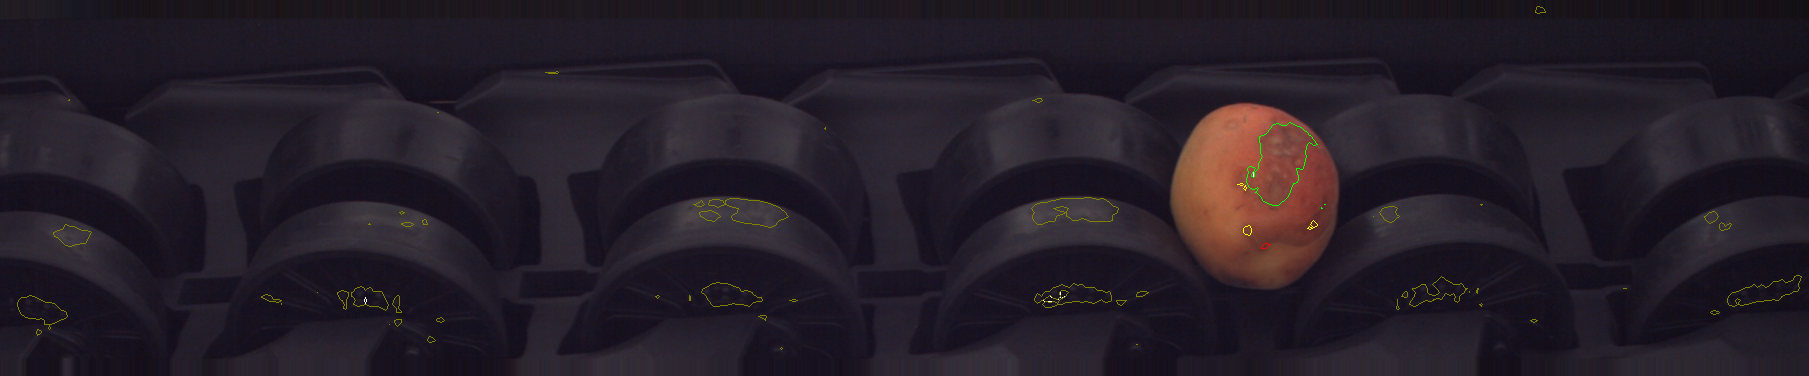
\includegraphics[scale=0.25]{img/marching_squares_00000052_00000001.png}
    \caption{Immagine scattata da macchina per la selezione della frutta senza elaborazioni applicate.}
\end{figure} 

L’implementazione di MS che è attualmente utilizzata dall’azienda deriva dalla libreria scikit-image che offre una versione seriale dell’algoritmo. Il metodo della libreria che viene chiamato è scritto in Python ma la parte principale è stata scritta in Cython.
Il codice in Cython deve essere compilato prima di essere eseguito, nel complesso però riduce i tempi di esecuzione rispetto all’equivalente in Python. Bisogna quindi considerare che il tempo totale di esecuzione di MS è stato già in parte ridotto dagli autori della libreria. \newline
In tutte le macchine sulle quali esegue il codice dell'azienda sono montate schede video di fascia alta per quanto riguarda le prestazioni, l'utilizzo di codice parallelo su GPU può essere quindi ampiamente sfruttato per ridurre i tempi di esecuzione e sollevare del carico la CPU su cui altrimenti ricadrebbe con esecuzioni seriali che in confronto sono estremamente dispendiose in termini di tempo.

\subsection{Obbiettivo}
L'obbiettivo concordato con l'azienda è quello di implementare una versione parallela su GPU (scheda video) dell'algoritmo Marching Squares, l'ottenimento di uno speedup rispetto alla versione utilizzata attualmente ovvero il metodo \verb|findContours| della libreria skimage sarebbe considerata un successo. \newline
Il software dell'azienda che attualmente richiama la funzione \verb|findContours| è scritta in Python, è necessario quindi riuscire trovare un metodo per poter sfruttare l'esecuzione parallela su GPU da Python, operazione non comune dato che solitamente i kernel Cuda sono lanciati da codice C o C++ ovvero a un livello di astrazione molto più basso di Python e con strutture dati come puntatori compatibili con quelli di Cuda. \newline
L'implementazione finale può essere rappresentata dallo schema in figura 3.4 ovvero una componente software che può essere richiamata direttamente da codice Python cioè un altro componente Python e delle parti aggiuntive di codice più a basso livello che siano in grado di lanciare ed eseguire codice sulla GPU in parallelo. L'unica parte della soluzione per cui la scelta del linguaggio da utilizzare risulta automatica è quella con cui si interfaccerà il codice dell'azienda, sarà quindi un modulo Python da cui poi si cercherà una strategia per arrivare all'esecuzione su GPU. \newline


\begin{figure}[H]
    \centering
    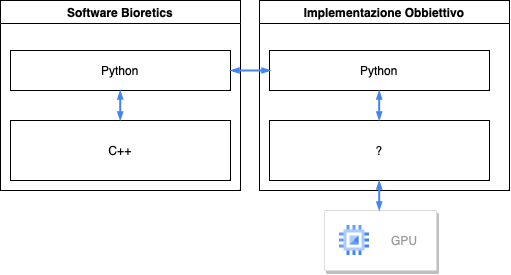
\includegraphics[scale=0.8]{img/Diagram_Python_GPU.drawio.png}
    \caption{Schema linguaggi utilizzati dal software dell'azienda e da utilizzate per la soluzione finale.}
\end{figure}

\section{Analisi implementazione skimage}
% analisi del metodo findContours
Il metodo \verb|findContours| di skimage composto da due fasi principali, nella prima viene richiamato un metodo \verb|_get_contour_segments| che trova le coordinate dei segmenti che costituiscono i contorni e una seconda parte in cui viene richiamato \verb|_assemble_contours| che dall'output di \verb|_get_contour_segments| unisce i segmenti che si intersecano sui bordi delle celle formando linee spezzate. \newline
% analisi parte core in Cython
Il metodo \verb|_get_contour_segments| è contenuto nel file \verb|_find_contours_cy.pyx| che è scritto in codice Cython, questo linguaggio è un superset di Python che permette di scrivere codice Python-like che effettua chiamate a funzioni C e può dichiarare tipi di dato del C, queste caratteristiche permettono al compilatore di generare codice ottimizzato per quanto riguarda i tempi di esecuzione rispetto all'equivalente in Python. \newline
% confronto prestazione Python<-->Cython
Non è semplice stabilire lo speedup del codice Cython rispetto al Python poiché il confronto dipende fortemente dalle strutture dati usate, il numero di funzioni C e python richiamate e altri fattori che influiscono in maniera significativa sulla differenza tra i tempi di esecuzione dei due linguaggi. Indubbiamente le chiamate a funzioni C da codice Cython introducono un overhead rispetto alla stessa chiamata effettuata da C e le funzioni Python impiegano un tempo sicuramente al massimo uguale e sicuramente non minore delle stesse funzioni richiamate da codice Python nativo. \newline
Nel complesso però se il codice Cython viene scritto con particolari accortezze nell'utilizzo di soli tipi di dato C e richiamando funzioni Python solo se indispensabili il codice che ne deriva risulta estremamente più veloce della versione Python, con tempi di esecuzione si avvicinano alla versione C che teoricamente può essere considerata un suo lower bound. Queste osservazioni sono riscontrabili graficamente nei risultati dei test generici riportati nella figura 3.5. 
\begin{figure}[H]
    \centering
    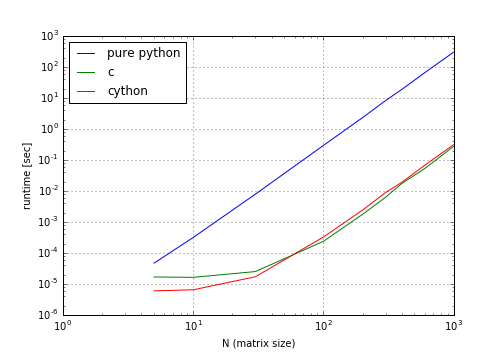
\includegraphics[scale=0.9]{img/cython-vs-c.png}
    % Image Source: http://ibm.co/20XSZ4F
    \caption{Grafico che mette in comparazione i tempi di esecuzione di Pyhon, C e Cython su un task di esempio. 
%TODO valutare di rifarlo manualmente o trovare altra fonte]
}
\end{figure} \newpage
Il codice del metodo Cython \verb|_get_contour_segments| risulta particolarmente ottimizzato in quanto utilizza unicamente variabili di tipo C e richiama una sola funzione di Python ovvero \verb|append| che può essere eseguita solitamente 0, 1 o al massimo 2 volte per ogni quadrato considerato. 
% osservazine --> tempi libreria già stretti
Il codice del metodo findContours può essere considerato quindi già particolarmente ottimizzato per essere un metodo Python, in quanto il suo tempo di esecuzione si può avvicinare molto ad una versione scritta in C. \newline
Con una immagine 511x95 il metodo findContours impiega in media circa \verb|0.0024s|**[NOTA: sulla mia macchina,  attendo test su server azienda per aggiornare valore e inserire specifiche macchina] %TODO specifiche macchina
ovvero neanche tre millesimi di secondo.

\section{Limiti della programmazione parallela}
% intro generale ai problemi della prog parallela
% spiegare che parte più dispendiosa in questo caso sarebbe caricamnto e scrittura dati visto che l'esecuzione di immagini di queste dimensioni è esigua
% osservazione --> dimensioni immagini
Nelle architettura Von Neumann la latenza introdotta dagli accessi alla memoria sono ordini di grandezza maggiori rispetto a un ciclo di clock e creano bottleneck che influiscono molto sui tempi di esecuzione di una versione di codice parallela.
Nell'applicazione pratica proposta dall'azienda le immagini da elaborare sono di dimensioni 511x95, con una versione parallela del Marching Squares idealmente ogni Cuda Core si occuperebbe di un singolo quadrato, con immagini di queste dimensioni servirebbero 47940 esecuzioni (ovvero il numero di quadrati) che una GPU di fascia alta riesce a coprire utilizzando tutti i suoi Cuda Core in parallelo reiterando il procedimento qualche volta. \newline
Indipendentemente da come può essere gestito il lancio e l'esecuzione del MS su GPU è indispensabile che l'immagine sia letta dalla memoria principale della macchina, caricata sulla memoria della GPU e in seguito il processo opposto sul risultato ottenuto sulla GPU.
Queste operazioni di trasferimento dati tra memorie sono estremamente dispendiose paragonate ai tempi di esecuzione delle istruzioni che un kernel Cuda può impiegare, questo rischia di essere uno dei maggiori problemi e limiti da affrontare per raggiungere uno speedup in quanto sicuramente una versione di codice parallelo ha il potenziale di essere più veloce del rispettivo seriale, ma al tempo del codice parallelo va sommato il tempo per caricare e scaricare i dati dalla GPU che influiranno in gran parte sul tempo di esecuzione finale. \newline
Se l'immagine fosse di dimensioni maggiori il tempo dovuto al bottleneck potrebbe essere ammortizzato maggiormente e la versione parallela avrebbe più margine su quella seriale, nel nostro caso invece la grandezza dell'immagine non richiede un tempo di esecuzione sufficientemente grande da far passare in secondo piano quello dei trasferimenti tra memorie. \newline
Il caso peggiore che si può presentare è che il rapporto dati da trasportare e le operazioni da effettuarci sia così sbilanciato che solamente il tempo di upload e download dei dati dalla GPU senza neanche contare il tempo di esecuzione del codice parallelo sia maggiore del tempo di esecuzione della versione seriale.


\section{Analisi versione seriale di MS}
La libreria \verb|scikit-image| (skimage) è un pilastro per quanto riguarda l'elaborazione di immagini in ambito Open-Source, è largamente utilizzata sia in piccoli progetti che in contesti industriali.  Il codice delle funzioni più utilizzate è particolarmente solido e ottimizzato pur mantenendo un'ampia compatibilità con una vasta lista di ambienti, tra queste funzioni ricade anche findContours che infatti presenta ottime prestazioni per essere una funzione seriale lanciata da Python.\newline
Dal codice di findContours che è riportato nella sezione di codice 1, proveniente dal file \verb|scikit-image/skimage/measure/_find_contours.py|, si può notare facilmente che vengono richiamati due metodi \verb|_get_contour_segments| e \verb|_assemble_contours| che costituiscono le due fasi di costruzione del risultato, la prima di pura ricerca algoritmica dei segmenti che costituiscono i contorni e la successiva di congiunzione dei contorni confinanti in linee spezzate. \\[10pt]
\noindent\rule[0.5ex]{\linewidth}{2pt}
\small{\textbf{Codice 1: Metodo find\_contours di scikit-image}} \\
\noindent\rule[0.5ex]{\linewidth}{1pt}

\lstset
{ %Formatting for code in appendix
    language=Python,
    basicstyle=\footnotesize,
    numbers=left,
    stepnumber=1,
    showstringspaces=false,
    tabsize=1,
    breaklines=true,
    breakatwhitespace=false,
}
\begin{lstlisting}
def find_contours(image,  level=None,  fully_connected='low', 
																		positive_orientation='low', *,  mask=None):

					...
					# parameters configuration
					...	

					segments = _get_contour_segments(
					 			image.astype(np.float64), 
					 			float(level),
								 fully_connected == 'high', 
					 			mask=mask)
    	contours = _assemble_contours(segments)
    	if positive_orientation == 'high':
        		contours = [c[::-1] for c in contours]
    	return contours
\end{lstlisting}
\noindent\rule[0.5ex]{\linewidth}{1pt} \\[10pt]
Il metodo \verb|_get_contour_segments| non è compreso nello stesso modulo di  \verb|find_contours| ma nel file \verb|scikit-image/skimage/measure/_find_contours_cy.pyx| che come si può notare termina con \verb|.pyx|, estensione che contraddistingue file contenenti codice Cython.  Come già accennato infatti \verb|_get_contour_segments| è stato scritto in Cython poiché è la parte computazionalmente più impegnativa dell'intero metodo \verb|find_contours|.  \newline
La maggior parte dei tipi di dati sono derivati dal C++ e altri dal Python come riportato nel seguente estratto di codice 2 del metodo Cython.  \newpage
\noindent\rule[0.5ex]{\linewidth}{2pt}
\small{\textbf{Codice 2: Estratto dal Metodo \_get\_contour\_segments di scikit-image}} \\
\noindent\rule[0.5ex]{\linewidth}{1pt}
\begin{lstlisting}
cimport numpy as cnp
cnp.import_array()
cdef extern from "numpy/npy_math.h":
    bint npy_isnan(cnp.float64_t x)
cdef list segments = []
cdef bint use_mask = mask is not None
cdef unsigned char square_case = 0
cdef tuple top, bottom, left, right
cdef cnp.float64_t ul, ur, ll, lr
cdef Py_ssize_t r0, r1, c0, c1
\end{lstlisting}
\noindent\rule[0.5ex]{\linewidth}{1pt} \\[10pt]
L'utilizzo dei questi tipi di dato C++ rispetto ai tipi Python permette di ottenere una compilazione più aderente alle necessità e volontà del programmatore che può specificare in modo preciso i tipi di dato di cui necessita. \newline
La porzione di codice più importante del metodo \verb|_get_contour_segments| è costituita da due cicli for annidati che scorrono tutta la matrice in input e considerano un quadrato di 4 celle ad ogni iterazione,  calcolano a quale dei sedici diversi tipi appartiene e aggiornano una struttura dati contenente tutti segmenti dei contorni trovati. \newline
Nell'aggiornamento dei segmenti trovati possono presentarsi tre diversi casi per quanto riguarda il numero di segmenti trovati:
\begin{itemize}
\item 0 segmenti da aggiungere: per i tipi 0 e 15 che sono quadrati con i 4 spigoli rispettivamente sotto e sopra la soglia di threshold non è necessario aggiungere alcun segmento poiché la relativa sezione dell'immagine in questione è completamente esclusa o inclusa in una certa classe,  non è attraversata quindi da segmenti del contorno come si può vedere dalla figura 3.6.
\begin{figure}[H]
\centering
\begin{floatrow}[1]
    \ffigbox[\FBwidth]{\caption{\small{Caso 0 e 15 dell'algoritmo Marching Squares.}}}{
\includegraphics[scale=0.27]{img/Case_0_15.svg.png}}
\end{floatrow}
\end{figure}
\item 2 segmenti da aggiungere: per i tipi 6 e 9 che sono quadrati con le due coppie di spigoli opposti in cui una è maggiore e una minore della soglia.  In questi due casi i segmenti da disegnare sono due,  ci sono due aree appartenenti ad una certa classe che hanno contorni vicini ma separati come osservabile nella figura 3.7.
\begin{figure}[H]
\centering
\begin{floatrow}[1]
    \ffigbox[\FBwidth]{\caption{\small{Caso 6 e 9 dell'algoritmo Marching Squares.}}}{
\includegraphics[scale=0.27]{img/Case_6_9.svg.png}}
\end{floatrow}
\end{figure}

\item 1 segmento da aggiungere: tutti gli altri tipi esclusi 0, 15, 6 e 9 hanno solamente un segmento che li attraversa in diverse modalità con diverse configurazioni di valori per i quattro spigoli del quadrato.  Rappresentano i casi più comuni di aree di contorno e   solitamente compongono la porzione maggiore di segmenti di cui sono costituite le linee spezzate con cui viene disegnato il contorno. Le 12 configurazioni sono rappresentate nella figura 3.8.
\begin{figure}[H]
\centering
\begin{floatrow}[1]
    \ffigbox[\FBwidth]{\caption{\small{Casi 1-5,7,8,10-14 dell'algoritmo Marching Squares.}}}{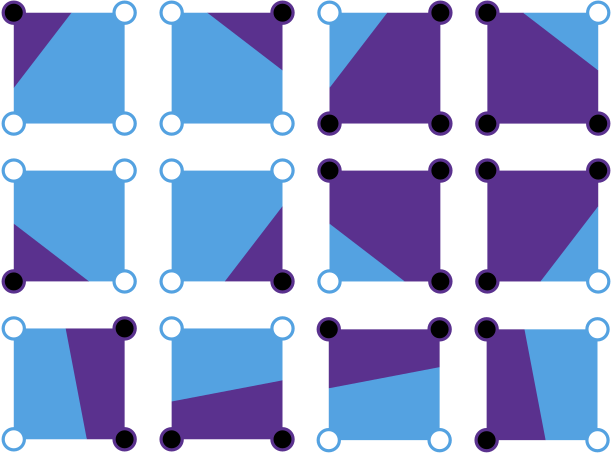
\includegraphics[scale=0.27]{img/Case_1seg.svg.png}}
\end{floatrow}
\end{figure}

\end{itemize}
% spiegare codice Cython per algoritmo MS
Ad ogni iterazione una volta definito a quale tipo appartiene un quadrato vengono aggiunti alla lista \verb|segments| i relativi segmenti trovati che possono essere 0, 1 o 2 come appena specificato.  Per ogni segmento trovato viene aggiunta a  \verb|segments| una tupla contenente altre due tuple in cui sono memorizzate le coordinate x e y del punto di inizio e fine del segmento, nel seguente estratto del metodo  \verb|_get_contour_segments| (Codice 3) viene riportata l'assegnazione delle coordinate per i punti che potranno essere aggiunti alla lista come estremi dei segmenti individuati.\newpage
\noindent\rule[0.5ex]{\linewidth}{2pt}
\small{\textbf{Codice 3: Estratto dal Metodo \_get\_contour\_segments di scikit-image}} \\
\noindent\rule[0.5ex]{\linewidth}{1pt}
\begin{lstlisting}
cdef inline cnp.float64_t _get_fraction(cnp.float64_t from_value,
                                        cnp.float64_t to_value,
                                        cnp.float64_t level):
    if (to_value == from_value):
        return 0
    return ((level - from_value) / (to_value - from_value))

top = r0, c0 + _get_fraction(ul, ur, level)
bottom = r1, c0 + _get_fraction(ll, lr, level)
left = r0 + _get_fraction(ul, ll, level), c0
right = r0 + _get_fraction(ur, lr, level), c1
\end{lstlisting}
\noindent\rule[0.5ex]{\linewidth}{1pt} \\[10pt]
Ognuno dei 16 casi deve essere gestito separatamente poiché le loro composizioni sono eterogenee per quanto riguarda i valori sugli spigoli e le coordinate da salvare.  
I segmenti vengono aggiunti alla lista  \verb|segments| tramite la funzione  \verb|append| che permette di costruire la lista di segmenti finale in modo incrementale senza dover conoscere a priori quale sarà la lunghezza finale della lista o quanti segmenti sarà necessario scrivere per ogni quadrato.  Per i casi 0 e 15 non è necessario aggiungere nessun segmento a segments quindi si passa direttamente all'iterazione successiva, per gli altri casi invece si aggiungono 1 o 2 segmenti in base al caso in cui si ricade.\\[10pt]
\noindent\rule[0.5ex]{\linewidth}{2pt}
\small{\textbf{Estratto dal Metodo \_get\_contour\_segments di scikit-image}} \\
\noindent\rule[0.5ex]{\linewidth}{1pt}
\begin{lstlisting}
# Manage case 0 and 15
if square_case in [0, 15]:
                continue

# Example for case 1-5, 7, 8, 10-14
if (square_case == 1): 
                # top to left
                segments.append((top, left))
# Example for case 6 and 9
elif (square_case == 6):
                 segments.append((left, top))
                 segments.append((right, bottom))
\end{lstlisting}
\noindent\rule[0.5ex]{\linewidth}{1pt} \newpage

% spiegare problema append per la parallelizzazione su GPU e le strutture dati
\subsection{Predisposizione alla parallelizzazione}
L'algoritmo Marching Squares essendo embarassingly parallel è teoricamente predisposto ad una parallelizzazione, le soluzioni parallele però hanno necessità specifiche che il codice seriale non ha bisogno di rispettare,  per riuscire a raggiungere questi requisiti partendo dal codice di  \verb|_get_contour_segments| è necessario effettuare radicali modifiche alle strutture dati utilizzate e al loro utilizzo. \newline
La principale criticità riscontrabile nel metodo è l'utilizzo di una lista e del metodo \verb|append| che non è possibile trasformare direttamente in ad esempio codice di un kernel Cuda poichè la dimensione finale della lista non è nota a priori e il metodo  \verb|append| non è disponibile in Cuda.  La funzione \verb|append| non potrebbe neanche essere utilizzata in una versione parallela ottimizzata poiché implica un accesso serializzato alla struttura dati lista per aggiungere il nuovo elemento in una nuova e ultima posizione della lista, questa operazione non può quindi essere effettuata contemporaneamente da più Cuda Core.  Per una versione parallela su GPU dato che il tipo dei quadrati e l'aggiunta dei segmenti verrebbe eseguita contemporaneamente sarebbe necessario avere un accesso indipendente e non vincolato alla risorsa di output su cui scrivere,  questo comporta la necessità di una struttura dati con un numero di posizioni già definito ma anche il numero di segmenti che ogni Cuda Core (ovvero per ogni quadrato valutato) necessita di scrivere.

% \chapter{Tentativi Svolti}
% valutare cambio nome
% spiegare tutti i tentativi svolti, 1 o più capitoli per ogni veersione o test
\chapter{Versione parallela con nvc++} 
La prima strategia esplorata consiste nel compilare il codice Cython con le ultime versioni del compilatore nvc++ che supporta dei flag per la parallelizzazione automatica su GPU.  Nvidia ha recentemente aggiornato \verb|stdpar,|  un flag che promette di riuscire a parallelizzare automaticamente codice C++ su GPU utilizzando il compilatore nvc++. \newline
Il processo parte da del codice Cython che tramite il proprio compilatore viene trasformato in codice C++,  a questo punto si compila il codice C++ utilizzando nvc++ e una serie di flag per la parallelizzazione su GPU tra cui \verb|stdpar|, infine si può richiamare il codice parallelizzato da Python tramite l'importazione del modulo generato. \newline
Il processo documentato da Nvidia è descritto in forma schematica nella figura 4.1.
\begin{figure}[H]
\centering
\begin{floatrow}[1]
    \ffigbox[\FBwidth]{\caption{\small{Schema di descrizione processo per utilizzo nvc++ in parallelizzazione codice Cython prodotto a Nvidia.}}}{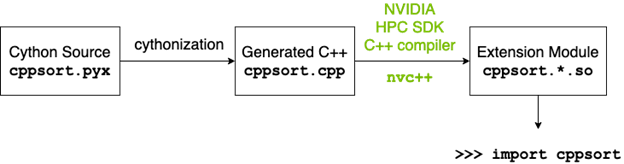
\includegraphics[scale=0.9]{img/extension-module.png}}
\end{floatrow}
\end{figure} \newpage

\section{Requisiti utilizzo nvc++}
Per poter utilizzare il flag stdpar con una versione aggiornata di nvc++ è necessario installare \verb|Nvidia High Performance Computing Software Development Kit (HPC SDK)| sulla macchina su cui verrà effettuata la compilazione e l'esecuzione. Le opzioni disponibili per ottenere HPC SDK sono installarlo direttamente sulla macchina oppure utilizzare un container Docker configurato da Nvidia con tutte le dipendenze di nvc++ installate. \newline
L'azienda Bioretics ha messo a disposizione un server con una scheda video RTX 2060 Super, per evitare tutte le problematiche legate alle dipendenze, le loro versioni e il loro mantenimento è stato valutato di utilizzare la soluzione con Docker. \newline
L'utilizzo del container docker fornito da Nvidia si è rivelato però particolarmente ostico da utilizzare poiché per il suo avvio è stata necessaria una configurazione molto articolata che non era descritta nella guida all'utilizzo. Per il corretto funzionamento del container e del compilatore nvc++ è stata necessaria una particolare configurazione che permettesse al container di utilizzare la scheda video e i suoi driver con permessi specifici. 
L'ambiente ottenuto sul server con la configurazione del container è rappresentato dalla figura 4.2.

\begin{figure}[H]
\centering
\begin{floatrow}[1]
    \ffigbox[\FBwidth]{\caption{\small{Schema componenti hardware e software sul server dell'azienda in seguito alla configurazione del container Nvidia HPC SDK.}}}{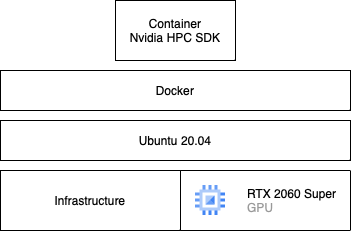
\includegraphics[scale=0.9]{img/Docker_HPC-SDK.drawio.png}}
\end{floatrow}
\end{figure} \newpage


\section{Potenziali risultati}

I risultati promessi da Nvidia con l'utilizzo di nvc++ e \verb|-stdpar| sembrano avere un potenziale altissimo, ma vanno ben contestualizzati ai task eseguiti e all'hardware utilizzato. \newline
I benchmarks effettuati dal team developer Nvidia sono sull'ordinamento di una serie di numeri e su iterazioni del metodo di Jacobi, entrambe sono due funzioni facilmente parallelizzabili, largamente studiate ed estremamente ottimizzate nelle implementazioni delle principali librerie.
Per ognuno dei due task sono state utilizzate 3 versioni:
\begin{itemize}
\item versione che utilizza la funzione seriale.
\item versione parallela su CPU che utilizza le policy di esecuzione parallela ed è compilata con g++.
\item versione parallela su GPU che utilizza sempre le policy di esecuzione parallela ma è compilata con nvc++ e l'opzione \verb|-stdpar|.
\end{itemize}

Nei test sull'ordinamento di numeri presentati in figura 4.3 è rappresentato lo speedup delle 3 versioni rispetto all'implementazione di Numpy della funzione .sort(). Si può notare uno speedup di circa 20x nel test con il numero maggiore di elementi della versione parallelizzata su GPU da nvc++ con -stdpar rispetto al .sort() di Numpy, risultato apparentemente molto promettente. Nei test con un basso numero di elementi risultano però migliori le versioni su CPU seriali e parallele, fenomeno dovuto all'overhead introdotto da un'esecuzione parallela su GPU che comporta il trasferimento di dati sulle memorie, questo problema è lo stesso discusso in precedenza in relazione alle dimensioni ridotte delle immagini utilizzate nell'applicazione reale oggetto di questa ricerca.

\begin{figure}[H]
\centering
\begin{floatrow}[1]
    \ffigbox[\FBwidth]{\caption{\small{Speedup ottenuto a confronto con Numpy nell'ordinamento di una sequenza di interi. I benchmarks su GPU sono stati eseguiti su un sistema con Intel Xeon Gold 6128 CPU, quelli su GPU invece su una NVIDIA A100.}}}{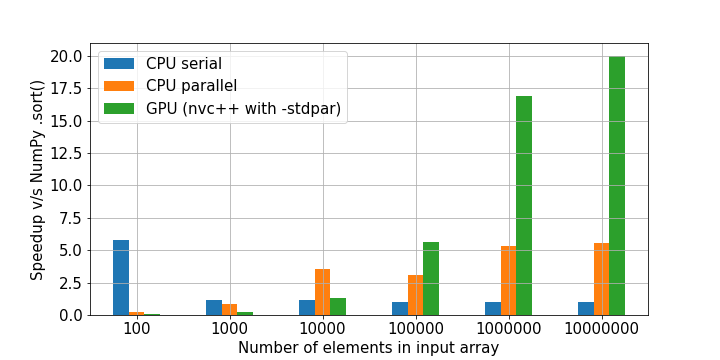
\includegraphics[scale=0.5]{img/speedup-vs-numpy-integer-sequence-1.png}}
\end{floatrow}
\end{figure} 

Nei test sulle iterazione del metodo di Jacobi il fenomeno riscontrato con .sort() non si presenta come osservabile nella figura 4.4, il test con il numero di elementi minore è di dimensioni nettamente maggiori rispetto a quello del test precedente ed è quindi già in grado di ammortizzare il costo impiegato per l'esecuzione parallela su GPU.
I risultati ottenuti in questi benchmarks sono ancora più eclatanti, tanto da insospettirsi sul fatto che siano realmente ottenibili anche su altre funzioni di utilizzo reale. \newline
Bisogna considerare infatti che tutti i risultati ottenuti in questi test con il compilatore nvc++ e la direttiva \verb|-stdpar| sono stati eseguiti su una macchina con componenti hardware di fascia altissima che permettono di avere una potenza di calcolo che è estremamente lontana da quella della maggior parte delle macchine utilizzate in ambito enterprise. Infatti la GPU utilizzata è una Nvidia A100 ovvero una scheda che si trova in configurazioni con decine di GB di memoria a costi di anche 10 volte maggiori a quelli di una GPU di fascia alta. \newline
Oltre all'hardware bisogna anche considerare che i task su cui sono stati effettuati i test comprendevano esclusivamente esecuzione di codice interamente parallelizzabile, strutturalmente quindi molto distante dal codice utilizzato come base per questo progetto.

\begin{figure}[H]
\centering
\begin{floatrow}[1]
    \ffigbox[\FBwidth]{\caption{\small{Speedup ottenuto a confronto con Numpy in iterazione di Jacobiano. I benchmarks su GPU sono stati eseguiti su un sistema con Intel Xeon Gold 6128 CPU, quelli su GPU invece su una NVIDIA A100.}}}{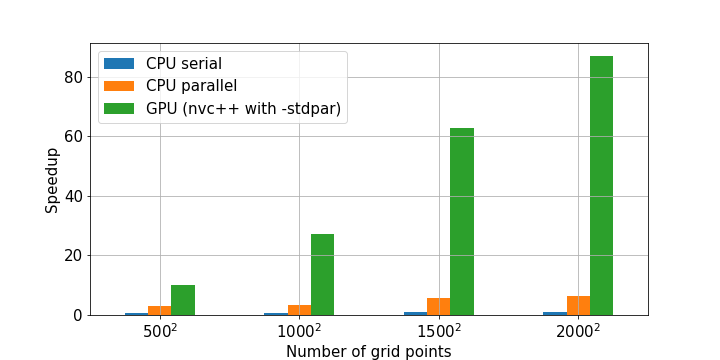
\includegraphics[scale=0.5]{img/speedup-vs-numpy-jacobi.png}}
\end{floatrow}
\end{figure} \newpage

\section{Marching Squares con nvc++ e -stdpar}
Il risultato migliore che potrebbe essere raggiunto è quello di riuscire a ottenere anche solo una frazione dello speedup riportato da Nvidia con nvc++ e -stdpar utilizzandoli con il codice Cython di skimage in cui è implementato MS.\newline
La strategia scelta per arrivare a questo risultato è quella di partire da una versione di codice basica e poi evolverla in quella finale a piccoli step in modo da risolvere in modo incrementale i problemi che inevitabilmente si presentano in implementazioni di questo tipo dove sono compresi codice di linguaggi diversi e compilatori complessi. \newline 
I risultati ottenuti dal team developer di Nvidia si sono subito rivelati un lontano traguardo da raggiungere con hardware di fascia media infatti testando lo stesso codice con cui erano stati effettuati i benchmarks sono stati ottenuti risultati che non erano neanche simili ma anzi peggiori delle versioni seriali e parallele su CPU. Ovviamente risulta difficile pensare di ottenere certi risultati sulla macchina su cui poi verrà utilizzato il codice con il proprio progetto se neanche il codice fornito da Nvidia perfettamente ottimizzato riesce a raggiungerli. Dato che per il successo del progetto però è sufficiente riuscire a parallelizzare su GPU anche solo una piccola parte del codice e ottenere uno speedup questa strada è stata considerata ancora valida. \newline
Il codice proposto da Nvidia era particolarmente semplice e da poche righe totali, la compilazione aveva quindi poche pretese, questo non vale per il codice Cython di skimage che comprende importazioni da librerie esterne e il loro utilizzo. Nel file \verb|setup.py| sono specificate tutte le direttive per la compilazione e viene gestito in collegamento di tutte le librerie necessarie. Per concludere senza errori la compilazione del codice di skimage è stato quindi necessario modificare la struttura e il contenuto delle opzioni di compilazione nel file \verb|setup.py| che viene passato a nvc++ per definire tutte le opzioni di compilazione e le librerie da includere. \newline
Il processo parte dalla trasformazione del codice Cython in C++ con \verb|cythonize|. \\[10pt]
\noindent\rule[0.5ex]{\linewidth}{2pt}
\small{\textbf{Cythonizzazione}} \\
\noindent\rule[0.5ex]{\linewidth}{1pt}
\begin{lstlisting}
$ cythonize -i _find_contours_cy.pyx
\end{lstlisting}
\noindent\rule[0.5ex]{\linewidth}{1pt} \\[8pt]
Il codice C++ ottenuto viene poi compilato con il seguente comando.\\[8pt]
\noindent\rule[0.5ex]{\linewidth}{2pt}
\small{\textbf{Compilazione con nvc++ e -stdpar}} \\
\noindent\rule[0.5ex]{\linewidth}{1pt}
\begin{lstlisting}
$ CC=nvc++ python setup.py build_ext --inplace
\end{lstlisting}
\noindent\rule[0.5ex]{\linewidth}{1pt} \\[10pt]
Il risultato di questo processo è un modulo importabile da python utilizzabile per rischiamare il metodo che verrà poi eseguito in parallelo su GPU. \newline 
%Una libreria necessaria al codice del MS di skimage è Numpy, perché fosse possibile importarla dal codice Cython è stato necessario aggiungerla alla lista delle librerie nel file \verb|setup.py|. \newline

\section{Problemi riscontrati}
Purtroppo tutti i tentativi effettuati non hanno portato ad una versione parallela funzionante su GPU. Il principale problema riscontrato è la complessità e disordine del codice C++ derivato dal processo di cythonizzazione del codice cython, il codice in output è infatti come dimensioni di ordini di grandezza maggiori. Da un centinaio di righe in cython il codice C++ risultante passa a decine di migliaia che risultano quindi ingestibili dato che ci andrebbero aggiunte manualmente le policy di esecuzione parallela per ogni singolo metodo della libreria standard che si vuole parallelizzare su GPU. Nei test effettuati anche inserendo le policy per la parallelizzazione l'esecuzione fallisce a causa delle strutture dati generate dalla cythonizzazione come puntatori a strutture che non sono riconosciute nativamente da C++ e quindi considerate come un insieme di byte. La parallelizzazione automatica su GPU di nvc++ con \verb|-stdpar| sul codice C++ derivato dal Cython si è rivelata quindi estremamente difficile da utilizzare con codice più complesso di quello proposto da Nvidia che comprendeva praticamente solo qualche funzione base della libreria standard C++. \newline
In seguito a queste conclusioni è stato valutato di non proseguire con questa strada ma intraprenderne una più complessa in termini di implementazione su cui però si può avere più controllo sul processo di parallelizzazione su GPU (descritto nel capitolo 5).

\chapter{Versione parallela con API Cuda-Python} 

\section{API Cuda-Python}
Cuda-Python è un progetto nato per unificare l'ecosistema di utilizzo di CUDA da Python con un insieme di interfacce a basso livello in grado di mettere a disposizione una copertura completa all'accesso da Python alle API dell'host CUDA. Il principale obbiettivo è quello di agevolare per i programmatori l'utilizzo di GPU Nvidia da codice Python.

\subsection{Requisiti Hardware e Software}
Per poter utilizzare le API Cuda-Python è necessario il CUDA Toolkit (dalla versione 12.0 alla 12.2) e predisporre una macchina che abbia una versione aggiornata sia di Python (da 3.8 a 3.11) che dei propri Driver Nvidia specifici per le proprie schede video. \newline
Dal CUDA Toolkit è richiesto solamente il componente NVRTC che è utilizzato a runtime per la compilazione di codice CUDA C++. \newline
La scheda video della macchina su cui viene utilizzato deve essere Nvidia ed essere compatibile con l'utilizzo di CUDA.

\subsection{CUDA Python workflow}
Il codice scritto in Cuda deve essere compilato per poter esser eseguito su una GPU, Python invece è un linguaggio interpretato che non necessita di una previa compilazione ma viene eseguito riga per riga. Per riuscire a richiamare un metodo Cuda da Python è necessario compilare il codice del device in PTX (Parallel Thread Execution) ed estrarne la funzione che potrà poi essere richiamata dall'applicazione python. PTX è una macchina virtuale per esecuzione di thread paralleli a basso livello che comprende un ISA (Instruction Set Architecture) ossia un insieme di istruzioni macchina. \newline
In pratica il codice del device (codice Cuda che verrà eseguito su GPU) viene scritto in una stringa python e compilato con NVRTC che è una libreria di compilazione runtime per CUDA C++. \newline
Il processo di esecuzione parallela del codice Cuda partendo da codice Python in generale consiste nell'utilizzo delle API per i Driver Nvidia per:
\begin{itemize}
    \item creazione manuale del \verb|context| CUDA su GPU
    \item allocazione manuale di tutte le risorse necessarie su GPU
    \item compilazione codice Cuda (contenuto in stringa Python) con NVRTC
        \begin{figure}[H]
        \centering
        \begin{floatrow}[1]
            \ffigbox[\FBwidth]{\caption{\small{Schema compilazione runtime con NVRTC di codice CUDA C++ da codice Python e output funzione compatibile PTX richiamabile da Python.}}}{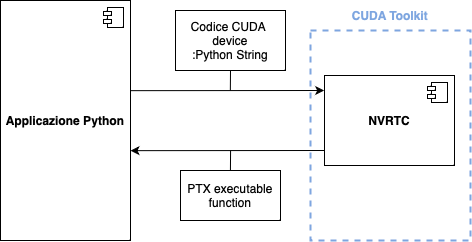
\includegraphics[scale=0.7]{img/Compilazione_NVRTC.png}}
        \end{floatrow}
        \end{figure} 
    \item caricamento dati da elaborare su GPU
    \item lancio codice compilato CUDA C++ su GPU
    \item recupero risultati da GPU 
\end{itemize} \newpage
\subsection{Utilizzo funzioni principali}
Per prima cosa vanno importati NVRTC e le API dei Driver dal pacchetto CUDA-Python come riportato nella seguente portzione di codice. Per copiare dati dall'host al device e viceversa è richiesto l'utilizzo di NumPy. \\[10pt]
\noindent\rule[0.5ex]{\linewidth}{2pt}
\small{\textbf{Importazione NVRTC, Driver API e NumPy}} \\
\noindent\rule[0.5ex]{\linewidth}{1pt}
\begin{lstlisting}
from cuda import cuda, nvrtc
import numpy as np
\end{lstlisting}
\noindent\rule[0.5ex]{\linewidth}{1pt} \\[10pt]
In seguito viene creato il programma a partire dal codice CUDA che può essere mantenuto in una stringa o portato in un file con estensione \verb|.cu| per mantenere ordine e chiarezza. Il programma deve poi essere compilato e dal risultato ne deve essere estratta la funzione PTX che potrà poi essere richiamata dal Python. In questo codice di esempio viene cercata una capacità di computazione di 75 con FMAD attivato.   \\[10pt]
\noindent\rule[0.5ex]{\linewidth}{2pt}
\small{\textbf{Creazione, compilazione e estrazione funzione PTX da codice CUDA C++}} \\
\noindent\rule[0.5ex]{\linewidth}{1pt}
\begin{lstlisting}
# Create program
err, prog = nvrtc.nvrtcCreateProgram(   str.encode(saxpy), 
                                        b"saxpy.cu", 
                                        0, [], []   )

# Compile program 
opts = [b"--fmad=false", b"--gpu-architecture=compute_75"]
err, = nvrtc.nvrtcCompileProgram(prog, 2, opts)

# Get PTX from compilation
err, ptxSize = nvrtc.nvrtcGetPTXSize(prog)
ptx = b" " * ptxSize
err, = nvrtc.nvrtcGetPTX(prog, ptx)
\end{lstlisting}
\noindent\rule[0.5ex]{\linewidth}{1pt} \newpage
Prima di poter utilizzare il PTX o eseguire qualsiasi cosa sulla GPU è necessario creare un CUDA context che è l'equivalente di un processo per la CPU. \newline
Successivamente è necessario inizializzare le API dei Driver per far in modo che i driver Nvidia e la GPU siano accessibili. Per assegnare la GPU principale della amcchina alla creazione \verb|context| va passato l'indicatore 0 alla funzione \verb|cuCtxCreate|. Con il \verb|context| creato si può procedere alla compilazione del CUDA kernel con NVRTC. \\[10pt]
\noindent\rule[0.5ex]{\linewidth}{2pt}
\small{\textbf{Inizializzazione Driver API e creazione context su device 0}} \\
\noindent\rule[0.5ex]{\linewidth}{1pt}
\begin{lstlisting}
# Initialize CUDA Driver API
err, = cuda.cuInit(0)

# Retrieve handle for device 0
err, cuDevice = cuda.cuDeviceGet(0)

# Create context
err, context = cuda.cuCtxCreate(0, cuDevice)
\end{lstlisting}
\noindent\rule[0.5ex]{\linewidth}{1pt} \\[10pt]
Con un CUDA \verb|context| creato sul device 0 si può caricare nel modulo il PTX generato in precedenza, un modulo è l'analogo per il device di librerie caricare dinamicamente. Più kernel posso essere contenuti all'interno di PTX, in seguito al carimento nel modulo è possibile estrarre uno specifico kernel con la funzione \verb|cuModuleGetFunction|. \\[10pt]
\noindent\rule[0.5ex]{\linewidth}{2pt}
\small{\textbf{Caricamento PTX come modulo ed estrazione funzione}} \\
\noindent\rule[0.5ex]{\linewidth}{1pt}
\begin{lstlisting}
# Get PTX
ptx = np.char.array(ptx)

# Load PTX as module data
err, module = cuda.cuModuleLoadData(ptx.ctypes.data)
ASSERT_DRV(err)

# Retrieve function
err, kernel = cuda.cuModuleGetFunction(module, b"saxpy")
ASSERT_DRV(err)
\end{lstlisting}
\noindent\rule[0.5ex]{\linewidth}{1pt} \newpage
In seguito tutti i dati a cui sarà necessario accedere dai kernel devono essere preparati e trasferiti sulla GPU, prima è necessario però allocare le risorse necessarie a contenere i dati utilizzando la funzione \verb|cuMemAlloc|. \newline
Una delle principali differenze tra Python e CUDA C++ è l'utilizzo di strutture dati differenti sia come tipo che livello di astrazione, Python nativamente non ha un concetto di puntatore ma la funzione \verb|cuMemcpyHtoDAsync| si aspetta \verb|void*| ovvero un puntatore senza un tipo specificato. La soluzione introdotta da Nvidia è quella di usare \verb|XX.ctypes.data| che recupera il valore del puntatore associato a \verb|XX|. \\[10pt]
\noindent\rule[0.5ex]{\linewidth}{2pt}
\small{\textbf{Creazione, allocazione e trasferimento dati su GPU}} \\
\noindent\rule[0.5ex]{\linewidth}{1pt}
\begin{lstlisting}
NUM_THREADS = 512  # Threads per block
NUM_BLOCKS = 32768  # Blocks per grid

a = np.array([2.0], dtype=np.float32)
n = np.array(NUM_THREADS * NUM_BLOCKS, dtype=np.uint32)
bufferSize = n * a.itemsize

hIn = np.random.rand(n).astype(dtype=np.float32)
hOut = np.zeros(n).astype(dtype=np.float32)

err, dInclass = cuda.cuMemAlloc(bufferSize)
err, dOutclass = cuda.cuMemAlloc(bufferSize)

err, stream = cuda.cuStreamCreate(0)

err, = cuda.cuMemcpyHtoDAsync(
   dInclass, hIn.ctypes.data, bufferSize, stream
)

\end{lstlisting}
\noindent\rule[0.5ex]{\linewidth}{1pt} \\[10pt]
Con i dati allocati e caricati i kernel sono pronti per essere lanciati, per farlo è necessario avere a disposizione gli indirizzi dei dati sul device per essere passati alle configurazioni di esecuzione. Per ottenere questi puntatori è possibile utilizzare \verb|int(dData)| che restituisce un tipo \verb|CUdeviceptr| e assegna un dimensione in termini di memoria con cui può essere memorizzato il valore utilizzando \verb|np.array()| . \newpage

\noindent\rule[0.5ex]{\linewidth}{2pt}
\small{\textbf{Recupero puntatori e allocazione parametri per funzione kernel}} \\
\noindent\rule[0.5ex]{\linewidth}{1pt}
\begin{lstlisting}
dIn = np.array([int(dInclass)], dtype=np.uint64)
dOut = np.array([int(dOutclass)], dtype=np.uint64)

args = [a, dIn, dOut, n]
args = np.array([arg.ctypes.data for arg in args], dtype=np.uint64)
\end{lstlisting}
\noindent\rule[0.5ex]{\linewidth}{1pt} \\[10pt]
Il kernel può essere lanciato con la funzione \verb|cuLaunchKernel| a cui vanno passati il modulo compilato del kernel e i parametri di configurazione per l'esecuzione. Lo stream creato in precedenza viene utilizzato sia per il trasferimento dei dati che per il lancio del codice del device, in questo modo il kernel inizia la sua esecuzione solamente quando è terminato il trasferimento di tutti i dati. Tutte le chiamate alle API e i lanci dei kernel su uno stream sono quindi effettivamente serializzati.\newline

\noindent\rule[0.5ex]{\linewidth}{2pt}
\small{\textbf{Lancio kernel}} \\
\noindent\rule[0.5ex]{\linewidth}{1pt}
\begin{lstlisting}
err, = cuda.cuLaunchKernel(
   kernel,
   NUM_BLOCKS,  # grid x dim
   1,  # grid y dim
   1,  # grid z dim
   NUM_THREADS,  # block x dim
   1,  # block y dim
   1,  # block z dim
   0,  # dynamic shared memory
   stream,  # stream
   args.ctypes.data,  # kernel arguments
   0,  # extra (ignore)
)
\end{lstlisting}
\noindent\rule[0.5ex]{\linewidth}{1pt} \\[10pt]
Dato che le chiamate alle API sono eseguite in sequenza si può richiedere la copia del risultato dal device all'host direttamente dopo il lancio del kernel, infatti la chiamata verrà risolta solo al termine dell'esecuzione del kernel. \newline
Prima di proseguire con altre chiamate per esempio a nuovi kernel è utilie richiamare la funzione \verb|cuStreamSynchronize| che mette in attesa la CPU fino a quando tutte le operazioni dello stream corrente non sono terminate. \newpage

\noindent\rule[0.5ex]{\linewidth}{2pt}
\small{\textbf{Trasferimento risultato da Device (GPU) a Host}} \\
\noindent\rule[0.5ex]{\linewidth}{1pt}
\begin{lstlisting}
err, = cuda.cuMemcpyDtoHAsync(
   hOut.ctypes.data, dOutclass, bufferSize, stream
)
err, = cuda.cuStreamSynchronize(stream)
\end{lstlisting}
\noindent\rule[0.5ex]{\linewidth}{1pt} \\[10pt]
Come ultima operazione è opportuno liberare le risorse allocate effettuando una pulizia della memoria l allocata su GPU e distruggendo sia lo \verb|stream| che il \verb|contex| creati. \newline

\noindent\rule[0.5ex]{\linewidth}{2pt}
\small{\textbf{Liberazione risorse}} \\
\noindent\rule[0.5ex]{\linewidth}{1pt}
\begin{lstlisting}
err, = cuda.cuStreamDestroy(stream)
err, = cuda.cuMemFree(dInclass)
err, = cuda.cuMemFree(dOutclass)
err, = cuda.cuModuleUnload(module)
err, = cuda.cuCtxDestroy(context)
\end{lstlisting}
\noindent\rule[0.5ex]{\linewidth}{1pt} \\[10pt]
Con queste ultime funzioni di pulizia si conclude l'introduzione ai comandi messi a disposizione delle API CUDA-Python che possono essere utilizzati per lanciare codice CUDA su GPU da codice Python. \newline
La versione di CUDA-Python utilizzata ovvero la 12.2.0 è ancora in evoluzione e potrebbe quindi essere aggiornata in futuro rendendo le funzioni precedenti o procedure descritte deprecate, è consigliato quindi consultare la pagina ufficiale di Nvidia per una documentazione aggioranta. \newpage

\subsection{Prestazioni dichiarate}
% benchmarks nvidia
Nvidia riporta i benchmark effettuati sul del codice di base ovvero tutte le istruzioni descritte in precedenza per l'utilizzo delle API con un semplice kernel CUDA che effettua semplici operazioni di algebra lineare chiamato SAXPY (Single-Precision A·X Plus Y). \newline
Ogni thread effettua solamente una operazione
\( a \cdot x + y \)
utilizzando un calore scalare e due valori letti da una coppia di array in input, scrive poi il risultato su un array di output.
La semplice implementazione CUDA utilizzata per i benchmark è la seguente. \\[10pt]
\noindent\rule[0.5ex]{\linewidth}{2pt}
\small{\textbf{Codice CUDA per device utilizzato nei benchmark}} \\
\noindent\rule[0.5ex]{\linewidth}{1pt}
\begin{lstlisting}
saxpy = """\
extern "C" __global__
void saxpy(float a, float *x, float *y, float *out, size_t n)
{
 size_t tid = blockIdx.x * blockDim.x + threadIdx.x;
 if (tid < n) {
   out[tid] = a * x[tid] + y[tid];
 }
}
"""
\end{lstlisting}
\noindent\rule[0.5ex]{\linewidth}{1pt} \\[10pt]
I risultati ottenuti dal team di Nvidia sono riportati nella tabella [ ] in cui si può notare come la versione C++ e Python appaiano estremamente simili come tempi di esecuzione sia per le pure esecuzioni dei kernel che per il tempo totale dell'applicazione. Si può osservare come la versione Python introduca un piccolo overhead riscontrabile nella differenza tra i due tempi di esecuzione totale che si discostano di qualche millisecondo. Le versioni kernel invece non hanno alcun tipo di differenza nei tempi di esecuzione, questo significa che una volta che i kernel sono lanciati la loro esecuzione non viene influenzata dal metodo utilizzato per lanciarli.


%\captionsetup{labelsep=newline,
   %           singlelinecheck=false,
      %        skip=0.333\baselineskip}
\newcolumntype{P}[1]{>{\centering\arraybackslash}p{#1}}

\begin{table}[h]
\centering
\setlength\tabcolsep{0pt} % let LaTeX figure out amount of inter-column whitespace
\caption{Comparazione tempi di esecuzione kernel e applicazione completa tra versione in C++ e Python.}
\label{turns}

\begin{tabular*}{\textwidth}{@{\extracolsep{\fill}} l *{3}{c} }
\toprule
\multicolumn{1}{c}{ } & \multicolumn{1}{c}{C++} & \multicolumn{1}{c}{Python} \\
\midrule
Kernel execution          & 352 µs    & 352 µs\\
Application execution & 1076 ms & 1080 ms  \\
\bottomrule
\end{tabular*}
\end{table}

%\section{Test API Cuda-Python}
\newpage
\section{Progettazione struttura codice parallelo}
La soluzione da sviluppare dovrà essere in grado di usufruire delle risorse GPU per i calcoli dell'algoritmo Marching Squares partendo da una chiamata ad un metodo Python per poter essere integrato al codice utilizzato da Bioretics. \newline
L'idea che comprende l'utilizzo delle API CUDA-Python è di creare un modulo python richiamabile dal codice dell'azieda che tramite le le API dei Driver Cuda riesca a caricare i dati, lanciare i kernel e recuperare il riusltato dalla GPU per poi restituirlo all'applicazione Python. \newline
Può essere quindi definito il nuovo quadro generale per questa soluzione che definisce il ponte tra il codice Python e il codice CUDA osservabile nella figura 5.2. \\[10pt]

\begin{figure}[H]
\centering
\begin{floatrow}[1]
    \ffigbox[\FBwidth]{\caption{\small{Schema utilizzo API CUDA-Python per utilizzo GPU da Python.}}}{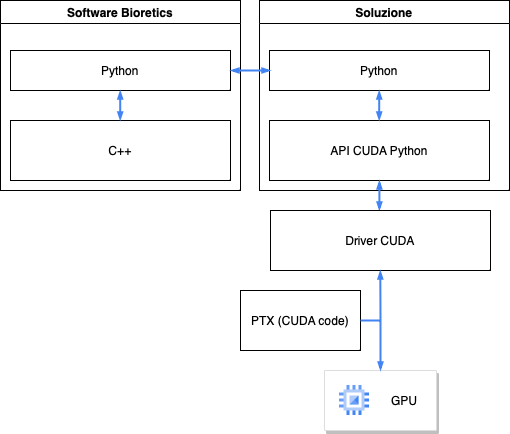
\includegraphics[scale=0.85]{img/Diagram_Python_GPU_API.drawio.png}}
\end{floatrow}
\end{figure} \newpage

La strategia ideata per il problema reale è di creare una funzione Python a cui poter passare il tensore Numpy in cui è memorizzata l'immagine su cui applicare Marching Squares e che restituisca i contorni individuati dall'algoritmo in una struttura dati compatibile nativamente con Python oppure Numpy. \newline
La funzine Python potrà essere importata nel codice dell'azienda ed essere quindi direttamente richiamabile, si occuperà quindi di interfacciarsi con le applicazioni esterno ad alto livello senza esporre l'implementazione a basso livello del codice CUDA e tutte le procedure necessarie al suo utilizzo. 
A causa però di alcuni parametri molto specifici relativi alla GPU utilizzata che vanno specificati per una corretta esecuzione ed utilizzo dell'hardware il codice non potrà rimanere invariato per macchine con schede video aventi caratteristiche particolarmente differenti.
I dati dell'immagine passata alla funzione andranno inevitabilmente trasferiti sulla memoria della GPU per poter essere elaborati dai kernel, andrà in seguito portato dalla memoria della scheda video a quella dell'host il risultato ottenuto con l'esecuzione parallela. %\newpage
\subsection{Strutture dati risultato}
La struttura dati utilizzata per il risultato dalla versione seriale di skimage è una lista, una delle principali sfide per una versione parallela è di riuscire a creare, mantenere e utilizzare strutture dati native C come alternativa. 
Una lista è una struttura dati estremamente flessibile che può essere creata senza dover specificare a priori la quantità di memoria che dovrà essere poi utilizzata in seguito a cui possono essere aggiunti elementi in modo incrementale. 
Oltre alla lista viene anche utilizzata la struttura dati tupla che può essere simulata in C con \verb|struct| ma dato che nella versione di skimage viene utilizzata una tupla contente due tuple non è possibile creare un array contenente questa struttura dati avendo la certezza che la memoria utilizzata sia contigua. Gli elementi di una tupla vengono disposti in modo contiguo in memoria solo se la loro dimensione è multipla di quella utilizzata dal compilatore altrimenti viene introdotto del padding tra un elemento e l'altro, nel nostro caso il tipo utilizzato è il \verb|double| che occupa 8 bytes e potrebbero quindi essere probabilmente disposti in sequenza in memoria senza l'aggiunta di padding. Per quanto riguarda una tupla contente due tuple però non è possibile stabilire con certezza come verranno disposti in memoria, non è quindi una soluzione ottimizzata utilizzare un array contentente queste tuple. \newline
Una struttura dati supportata nativamente da C che possa sostituire una lista di tuple contenetei tuple di double sono un inisieme di 4 array, non è la sola a poter esser utilizzata ma è quella che ottimizza maggiormante l'utilizzo dello spazio dei propri elementi, dello spazio totale e all'accesso alle posizioni specifiche. Ovviamente mantenere 4 array disconnessi fisicamente ma uniti solo a livello logico sono molto più delicati e richiedono una attenzione maggiore per essere mantenuti consistenti, l'idea è di memorizzare i 4 double utilizzando un unico indice per accedere alla stessa rispettiva posizione nei 4 array C. \newline
La struttura dati mantenuta su Python da skimage è rappresentata nella figura 5.3 e quella che verrà utilizzata per la versione parallela nella figura 5.4. \newline



\begin{figure}[H]
\centering
\begin{floatrow}[1]
    \ffigbox[\FBwidth]{\caption{\small{Insieme di strutture dati utilizzate per la versione Python di skimage.}}}{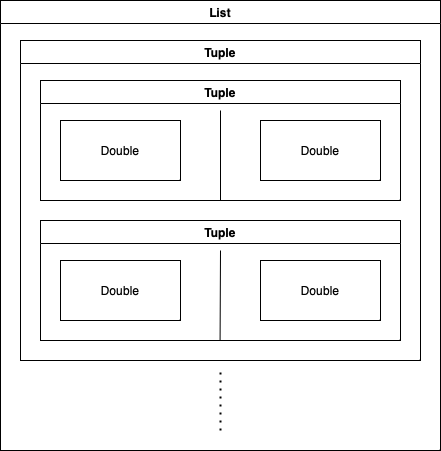
\includegraphics[scale=0.6]{img/list_tuple_double.drawio.png}}
\end{floatrow}
\end{figure}
\begin{figure}[H]
\centering
\begin{floatrow}[1]
    \ffigbox[\FBwidth]{\caption{\small{Insieme di strutture dati utilizzate per la versione parallela.}}}{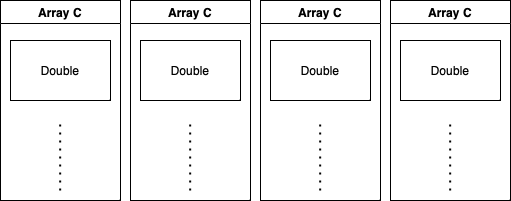
\includegraphics[scale=0.6]{img/4array.drawio.png}}
\end{floatrow}
\end{figure} 

Gli array C di tipo double consentono di avere la certezza che i vari elementi dello stesso array siano memorizzati in modo contiguo in memoria. Questa caratteristica è di fondamentale importanza per le operazioni in memoria a cui saranno sottoposti come scritture, letture, trasferimenti da e su GPU che privilegiano accessi coalizzati ad aree contigue che sfruttano interamente i bus invece che solo parzialmente ricorrendo in una penalizzazione sui tempi. \newpage

\section{Progettazione kernel Cuda}
La fase di progettazione dei kernel Cuda è quella che ha richiesto il maggior studio e pianificazione in quanto la parallelizzazione del codice skimage sfrutta una struttura dati per l'output che non è utilizzabile in una versione parallela. \newline
Dopo una veloce analisi del codice seriale è chiaro che un singolo kernel non sarà sufficiente ma saranno necessari diversi kernel da lanciare in sequenza per riuscire a replicare il funzionamento del codice seriale in parallelo. \newline
\subsection{Kernel required\_memory}
Dato che per utilizzare gli array è necessario definire al momento della loro creazione la dimensione che occuperanno in memoria è necessario stabilire quante posizioni degli array verranno utilizzate per una certa immagine. Il primo kernel quindi si occuperà di calcolare in modalità parallela il numero di segmenti che dovranno essere memorizzati con l'algoritmo Marching Squares per ogni singolo quadrato che andrà esaminato.
Per ogni quaderato composto da 4 valori confinanti verranno stabilite quante posizioni dell'array occuperanno. \\[10pt]

\noindent\rule[0.5ex]{\linewidth}{2pt}
\small{\textbf{Codice CUDA kernel required\_memory}} \\
\noindent\rule[0.5ex]{\linewidth}{1pt}
\begin{lstlisting}
size_t r0 = blockIdx.y * blockDim.y + threadIdx.y;
size_t c0 = blockIdx.x * blockDim.x + threadIdx.x;
    /*
    ...
    */
if (square_case == 0 || square_case == 15){
    // 0
    result_required_memory[ r0 * width + c0 ] = 0;
}
else if (square_case == 6 || square_case == 9){
    // 2
    result_required_memory[ r0 * width + c0 ] = 2;
}
else {
    // 1
    result_required_memory[ r0 * width + c0 ] = 1;
}  
\end{lstlisting}
\noindent\rule[0.5ex]{\linewidth}{1pt} \\[10pt]

L'output di questo primo kernel sarà quindi un vettore di dimensione pari al totale dei quadrati analizzabili dell'immagine che conterrà nella posizione rispettiva all'immagine un valore da 0 a 2 che indica quanti segmenti sarà necessario memorizzare per quel preciso quadrato. come mostrato nella figura 5.5.
\begin{figure}[H]
\centering
\begin{floatrow}[1]
    \ffigbox[\FBwidth]{\caption{\small{Array C risultato dell'esecuzione del kernel required\_memory.}}}{
\includegraphics[scale=0.8]{img/kernel1_out.drawio.png}}
\end{floatrow}
\end{figure} 
Non abbiamo ancora a disposizione il numero di posizioni totali necessarie per memorizzare tutti i segmenti, il vettore va immaginato di dimensioni elevate tali per cui una somma dei suoi elementi in versione seriale sia in relazione alla versione parallela estrememente lenta. Sono quindi necessarie altre operazioni parallele per poter ottenere la somma di tutti gli elementi dell'array generato da questo primo kernel. \newpage

\subsection{Kernel reduce}
Per calcolare la somma di tutti gli elementi dell'array output del kernel required\_memory è necessario effettuare una operazione di riduzione che è possibile parallelizzare. \newline
La reduce viene effettuata utilizzando ad ogni passaggio un numero di Cuda Core pari alla metà del numero di elementi rimasti, ad ogni iterazione ogni Cuda Core somma al valore presente nella posizione dell'array rispettiva al proprio indice (\verb|threadIdx.x|) il valore nella metà superiore corrispondente alla stessa posizione ovvero \verb|(blockDim.x / 2) + threadIdx.x|. \newline In questo modo il risultato può essere ottenuto in \(O(log_2 n)\) passi paralleli come mostrato nell'immagine 5.6.

\begin{figure}[H]
\centering
\begin{floatrow}[1]
    \ffigbox[\FBwidth]{\caption{\small{Operazione di reduce.}}}{
\includegraphics[scale=0.8]{img/reduce.drawio.png}}
\end{floatrow}
\end{figure} 
Ad ogni passo si dimezzano come il numero di elementi restanti anche il numero di thread utilizzati, questo significa che ci saranno thread che resteranno senza alcun lavoro da svolgere. \newline
Una accortezza è quella di lanciare il kernel con un numero di thread che siano la metà della lunghezza dell'array in modo che per almeno il primo passo tutti quanti i thread siano utilizzati. \newline
Tra un passo e l'altro è necessario richiamare la funzione \verb|__syncthreads()| che attende tutti i thread in esecuzione per evitare che i diversi thread lavorino a passi differenti della riduzione rendendo incosistenti le letture sull'array.  \newpage
\noindent\rule[0.5ex]{\linewidth}{2pt}
\small{\textbf{Codice CUDA kernel sum-reduce}} \\
\noindent\rule[0.5ex]{\linewidth}{1pt}
\begin{lstlisting}
const size_t lindex = threadIdx.x;
const size_t bindex = blockIdx.x;
const size_t gindex = blockIdx.x * blockDim.x + threadIdx.x;
size_t bsize =  blockDim.x / 2;
temp[lindex] = required_memory[gindex];
__syncthreads();

while( bsize > 0 ){
    if( lindex < bsize && (lindex+bsize)<n ){
        temp[lindex] += temp[lindex+bsize];
    }
    bsize = bsize / 2;
    __syncthreads();
}
if(0==lindex){
    result_reduce[bindex] = temp[0];
} 
\end{lstlisting}
\noindent\rule[0.5ex]{\linewidth}{1pt} \\[10pt]

In seguito alla lettura iniziale dalla memoria principale della GPU tutte le operazioni vengono effettuate successivamente sono sulla memoria condivisa della scheda video che richiede tempi molto più rapidi per le operazioni di lettura e scrittura. \newline
Lo scalare ottenuto con l'ultimo passo viene copiato nella locazione di memoria del risultato dal thread 0. 
Ogni blocco di thread ottiene quindi la somma dei valori corrispondenti alle loro posizioni, una volta riportati questi risultati parziali sull'host è necessario effettuare un'ulteriore operazione di somma su di questi per ottenere il risultato finale. In questo caso però il numero di blocchi necessari per elaborare tutto l'array non è sufficientemente grande da garantire una convenienza in termini temporali per il lancio di un kernel parallelo su GPU rispetto a effetture la somma degli elementi con una funzione ottimizzata come \verb|.sum()| fornita da Numpy. \newline
Il risultato finale che unisce i risultati parziali degli altri blocchi è ottenuto con il seguente codice Python dall'host.

\noindent\rule[0.5ex]{\linewidth}{2pt}
\small{\textbf{Codice host in Python per somma risultati parziali del kernel reduce}} \\
\noindent\rule[0.5ex]{\linewidth}{1pt}
\begin{lstlisting}
np_result_reduce = np.array(result_reduce) 
N_RES = np_result_reduce.sum()
\end{lstlisting}
\noindent\rule[0.5ex]{\linewidth}{1pt} \\[10pt]

\subsection{Kernel exclusive scan (prescan)}
Una volta ricavato quanto sia il totale di segmenti che andranno memorizzati manca ancora un componente per poter lanciare il kernel che eseguirà Marching Squares. Ora che possiamo allocare tutto lo spazio necessario e che tutti i thread che eseguiranno MS avranno uno spazio sufficiente per scrivere i segmenti trovati è necessario definire in quali posizioni della memoria riservata ognuno di loro dovrà scrivere. \newline
Esiste una funzione da applicare ad un array che calcola esattamente il risultato di cui abbiamo bisogno ovvero un array che contiene le posizioni in cui il thread corrispondente alla posizione in cui è salvata deve scrivere i suoi risultati.
Questa funzione è la exclusive scan chiamata anche prescan, calcola tutti i prefissi di un array in base ad una operazione data che nel nostro caso sarà l'operatore binario di somma. \newline
La exclusive scan è caratterizzata dal fatto che nella prima posizione dell'array risultato venga messo il valore dell'elemento neutrale dell'operazione utilizzata che è lo zero per la somma, tutti i valori del risultato sono quindi spostati di una posizione verso destra e l'ultimo valore dell'array in input non viene considerato. Un esempio di array risultato di una exclusive scan è riportato nella figura 5.7.

\begin{figure}[H]
\centering
\begin{floatrow}[1]
    \ffigbox[\FBwidth]{\caption{\small{Vettori di input e output della funzione di exclusive scan.}}}{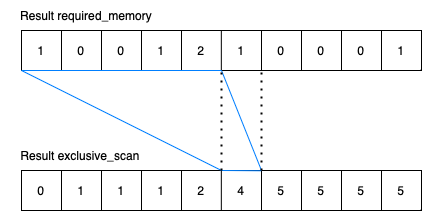
\includegraphics[scale=0.8]{img/prescan.drawio.png}}
\end{floatrow}
\end{figure} 
Il risultato di una exclusive scan su un array per le sue proprietà è già pronto per essere utilizzato per lo scopo desiderato infatti in ogni posizione è contenuta la posizione in cui andrà scritto il rispettivo valore. Rispetta anche gli indici degli array infatti la prima posizione indicata in cui scrivere è lo 0, per quelle successive invece il valore della posizione non considera quanti segmenti andranno scritti da quel thread ma solo quelli precedenti che è corretto dato che è necessario saper solo da dove iniziare a scrivere.
Sono presenti posizioni ripetute nel vettore in output, il risultato è corretto in quanto l'indice della prossima posizione in cui scrivere non deve variare se i rispettivi thread non hanno alcun segmento da scrivere. I thread che invece dovranno scrivere 2 segmenti dovranno scriverli consecutivamente partendo dalla posizione specificata nel risultato dell'exclusive scan. \newpage

Per effettuare l'operazione di exclusive scan su un array di grandi dimensioni un singolo kernel non è sufficiente.
Sono necessari infatti un totale di 3 kernel differenti per comporre il vettore finale in modalità parallela:
\begin{itemize}
    \item prescan (exclusive scan)
    \item prescan\_small  (exclusive scan small)
    \item add
\end{itemize}
Non è possibile effettuare tutti i passaggi necessari in un unico kernel poichè ...

\subsubsection{kernel prescan}
\subsubsection{kernel prescan\_small}
\subsubsection{kernel add}
% descrizione 3 kernel per la reduce

% schema finale per calcolo memoria, reduce ecc

% tecnica innovativa exclusive scan

\newpage
\section{Implementazione}
\subsection{Implementazione modulo python}
\subsection{Implementazione kernel}
% problema dell'append in Cython non convertibile direttamente in Cuda ==> utilizzo array
% tecnica innovativa exclusive scan

%problema illegal access error
    % # For Illegal memory access error
    %     err, = cuda.cuCtxSynchronize()
    %   ASSERT_DRV(err)
    % err, = cuda.cuStreamSynchronize(stream)
    %ASSERT_DRV(err)
\section{Risultati ottenuti}


\chapter{Risultati a Confronto}
% speedup, ecc.. In sostanza si descrivono e commentano i grafici ottenuti
% se si vuole misurare tempo di 2° paarte di find_contours() poi meglio lasciare distinte le due misurazioni (lib completa e assemble contours) in modo di dare a chi legge la possibilità di valutare la precisione non perfetta della misura
% mostrare overhead lancio kernel da python rispetto a C

\chapter{Conclusioni}
% speculare all'abstract, si dicono le stesse cose ma invece che "andremo a fare"  si dirà "abbiamo fatto"
% keyword: ABBIAMO fatto

\end{document}
